% Chapter 6

\chapter{Conclusion} % Write in your own chapter title
\label{Chapter:Conclusion}
\lhead{Chapter 6. \emph{Conclusion}} % Write in your own chapter title to set the page header

This thesis describes \steel, the STastical sEmi-Empirical modeL, a model designed to use the empirical technique in a new fashion to make a predictions that are complementary to traditional discrete models. The foremost problem concerning galactic modelling on a cosmological scale is one of constraint in overwhelmingly complex systems. Complexity and uncertainty is built into systems form all contributing aspects, from the dark matter simulations \cite[e.g.]{vandenBosch2018DisruptionFiction}, to observations \cite[e.g.]{Bernardi2017ComparingLight, Lapi2017StellarEquation, Leja2019AnSurvey}. Techniques have been developed to try to reduce the impact of these effects for example:
\begin{itemize}
    \item Abundance matching is able to create a mapping between any stellar mass function and halo mass function. In doing so it provides a consistent framework to use for galactic modelling for a given dark matter model.
    \item Continuity modelling uses the growth of the stellar mass functions to avoid conflicts between observed star formation rates and cosmological stellar mass densities. 
\end{itemize}

The mantra `publish or perish' combined with a hostility between different modelling techniques creates an environment where researchers are pushed to report positive and new results. It is unsurprising then that the number of papers that report new techniques or fits to data far outweigh those models which deconstruct the techniques to understand how are models work and document their limitations \cite[e.g.][]{vandenBosch2017DissectingSimulation, vandenBosch2018DisruptionFiction, Asquith2018CosmicModels}. We are driven to tune multi parameter systems and over-fit or be out competed by those who do.

\steel was designed as a reaction to this gap in cosmological modelling. Through flexible modelling and prioritising the understanding of systematics and internal self consistency above that of fitting new features we find a unique perspective. \steel is therefore not a physical model and in this way is the antithesis of high resolution single galaxy or cluster simulations such as FIRE \cite{Hopkins2018FIRE-2Formation}. Galaxy modelling is often seen as a spectrum from hydrodynamical, though semi-analytic and semi-empirical to mock catalogues produced via HOD. In this regime \steel can be thought of as occupying a space between traditional semi-empirical and HOD modelling, we retain the ability to track galaxy populations in redshift but forgo the tracking of discrete objects from step to step. Despite the antithetical nature of \steel to the hydrodynamical and non-statistical models it is not adversarial, use in conjunction with other techniques is likely its best use case. 

\section{Pros and Cons of \steel as a Galaxy Model}
%successes of STEEL where other models fall down
%what if theoretically impossible in steel that other models can do

\steel has had the following major successes:
\begin{itemize}
    \item Reproduction of the statistical distribution of satellite galaxies in dark matter halos over a broad redshift range.
    \item Identification of the inconstancy between certain stellar mass functions and dark matter accretion histories produced by \LCDM cosmologies.
    \item Derivation of the star formation rate from a new halo centric approach, consistent with cutting edge observations.
\end{itemize}
Each of these directly stem from the statistical dark matter accretion history, however, this technique looses individual galaxies that could be tracked though hydrodynamical, semi-analytic, and traditional semi-empirical models.

\steel is not a physical model it is a systematic model, it is not within the remit of \steel to predict but to apply predictions to full simulations and draw transparent conclusions about the way assumptions and models propagate into observed populations. Furthermore, Chapter \ref{Chapter:GalPairs} shows the potential of this systematic technique to track how changes to input propagate to output in a complex system, as shown with the pair fractions. Finally, using morphological models, we are able to show how we can test multiple models to understand how each effects the resultant population individually.

\section{Impact of \steel}
%how impactful is the work done with STEEL on the wider field?

\subsection{Modelling}

Creating another cosmological model acting on a discrete dark matter background has little value to add with several good models already existing in empirical, \cite[e.g.][]{Rodriguez-Puebla2017ConstrainingProperties, Moster2018Emerge10, Behroozi2019UniverseMachine:010, Zavala2012}, analytic \cite[e.g.][]{Somerville2015StarGas, Guo2011FromCosmology, Fontanot2007ReproducingCosmogony, Zoldan2019TheEvolution} and, hydrodynamical \cite{Springel2018FirstClustering, Hopkins2018FIRE-2Formation, McAlpine2015TheCatalogues} regimes. The systematic statistical approach can be used to complement these models in two ways:
\begin{itemize}
    \item Pre-Processing: 
    \begin{itemize}
        \item \steel can be used to test the validity of the combinations of input data. For example as in Chapter \ref{Chapter:GalGrowth} check the self-consistency of a dark matter assembly and a stellar mass function before they are used in a semi-analytic or hydrodynamic model.
        \item \steel can test simplified versions of theoretical physical models to check if they have the desired outcome on population before they are committed to more computationally intensive models
    \end{itemize}
    \item Cosmological extrapolation: 
    \begin{itemize}
        \item Using the same dark matter cosmology and input mass functions \steel can be used to extrapolate predictions to a larger scale. For example \steel matches satellite distributions in both massive cluster predictions and the Illustris TNG simulation. This gives an indication that the hierarchical collapse models in TNG are correct and will extrapolate well to large surveys once larger simulations are feasible.
    \end{itemize}
\end{itemize}
\subsubsection{Data}

We have shown how \steel can be used to combine data with a given cosmology to: predict consistency, satellite distributions, and star formation rates. This has been used to add weight to the claims made about light profiles from \citet{Bernardi2017ComparingLight} and the star formation rates from \citet{Leja2019AnSurvey}. In each of the aforementioned works problems are identified in current data analysis and more advanced data fitting routines are used, in the case of \citet{Bernardi2017ComparingLight} this involves the improved PyMorph photometery and systematic over subtraction of sky background in SDSS to better fit the observed luminosities, and in \citet{Leja2019AnSurvey} the use of prospector that can fully account for the starformation histories to better fit the starformation rate. \steel has currently worked on these problems after the fact, fully realised it could be an integral part of data fitting routines.

\section{Future of \steel in Galactic Astrophysics}
%How can we build on what we have done?

The future of \steel and potentially the future of statistical semi-empirical modelling now relies on communication of the advantages (and disadvantages) of the technique. We have begun to build collaboration around the model with several other empirical modellers, dark matter physicists, observers (both survey designers and data analysts), as well modellers that use semi-analytic and hydrodynamic models. The reception to \steel has been widely positive with many intrigued by its unique capabilities. The most notable group involved is the EUCLID consortium, working with EUCLID steel has the potential to have preferential access to the earliest survey data, and if developed correctly could be used in conjunction with the data analysis pipelines to ensure the routines used to fit the observations are consistent with cosmological theory.

PJG outlined the methodology to create \steel along side a 4 year development plan for a fellowship proposal\footnote{Unfortunately unsuccessful, the proposal and related documents are included in full in Appendix \ref{Appx:HF}.}. In this plan the future of \steel was separated into two complementary pathways, a data fitting tool and a galaxy modelling tool. 

\subsubsection{Data fitting tool}

HOD modelling is commonly used to create mocks that used to give an indication of what types of objects a given mission can expect to observe. Using relationships such as the SMHM relation, two point correlation function, black hole - velocity dispersion, e.t.c... simulated 'light cones' can be built up and using estimated sensitivities the extent of observable objects estimated. This kind of modelling is done prior to first light and far separated from the actual photons to be received. With \steel we can do better, getting closer to the real data and having active feedback in the data fitting processes contributing proactively to the scientific goals of a mission. 

Using Figure \ref{fig:Full_Mod_Toon} we show how \steel can be positioned to become a key element of observational fitting bringing theory and observation much closer than ever before. \textcolor{MPLgreen}{The observational inputs (green) are twofold, the survey i.e. the collected photons which are the only constant in the system, secondly the observational fits that are used to derive physical attributes from the collected photons. In this example the survey and fits generate the stellar mass function (SMF).}\textcolor{MPLred}{Secondly, the dark matter cosmology is input, it is worthy of note that the exact cosmological parameters may also influence the fits used. As described throughout this thesis \steel uses halo mass functions (HMF), halo substructures, and halo growth histories that are tuned to a dark matter simulation which are then turned into the statistical dark matter accretion history.} Excluding the actual collected photons the elements described thus far are all incredibly flexible and often well parameterised and documented. \textcolor{MPLblue}{The final input element is the modelling Traditionally, this is often computationally intensive, time consuming, and often degenerate; the empirical approach, especially as used within \steel, offers solutions to these problems being computationally light, fast, and transparent.} As described in Chapter \ref{Chapter:GalGrowth} using Figure \ref{fig:SFRDerevation_Cartoon} we can derived the star formation rate and bimodality using a combination of \textcolor{MPLgreen}{observation}, \textcolor{MPLred}{cosmology}, and \textcolor{MPLblue}{modelling}. By comparing derived products from fitted observations and modelled properties we can create a check that all fits used are self consistent and evolve appropriately with time within a given cosmology e.g.
\begin{itemize}
    \item Satellite galaxy distribution
    \item Pair fraction
    \item Star formation rate / cosmological star formation density
    \item Star formation - stellar mass function continuity
    \item Galaxy bimodality
    \item Galaxy morphology
    \item Active galactic nuclei background 
\end{itemize}
\begin{figure}[t]
    \centering
    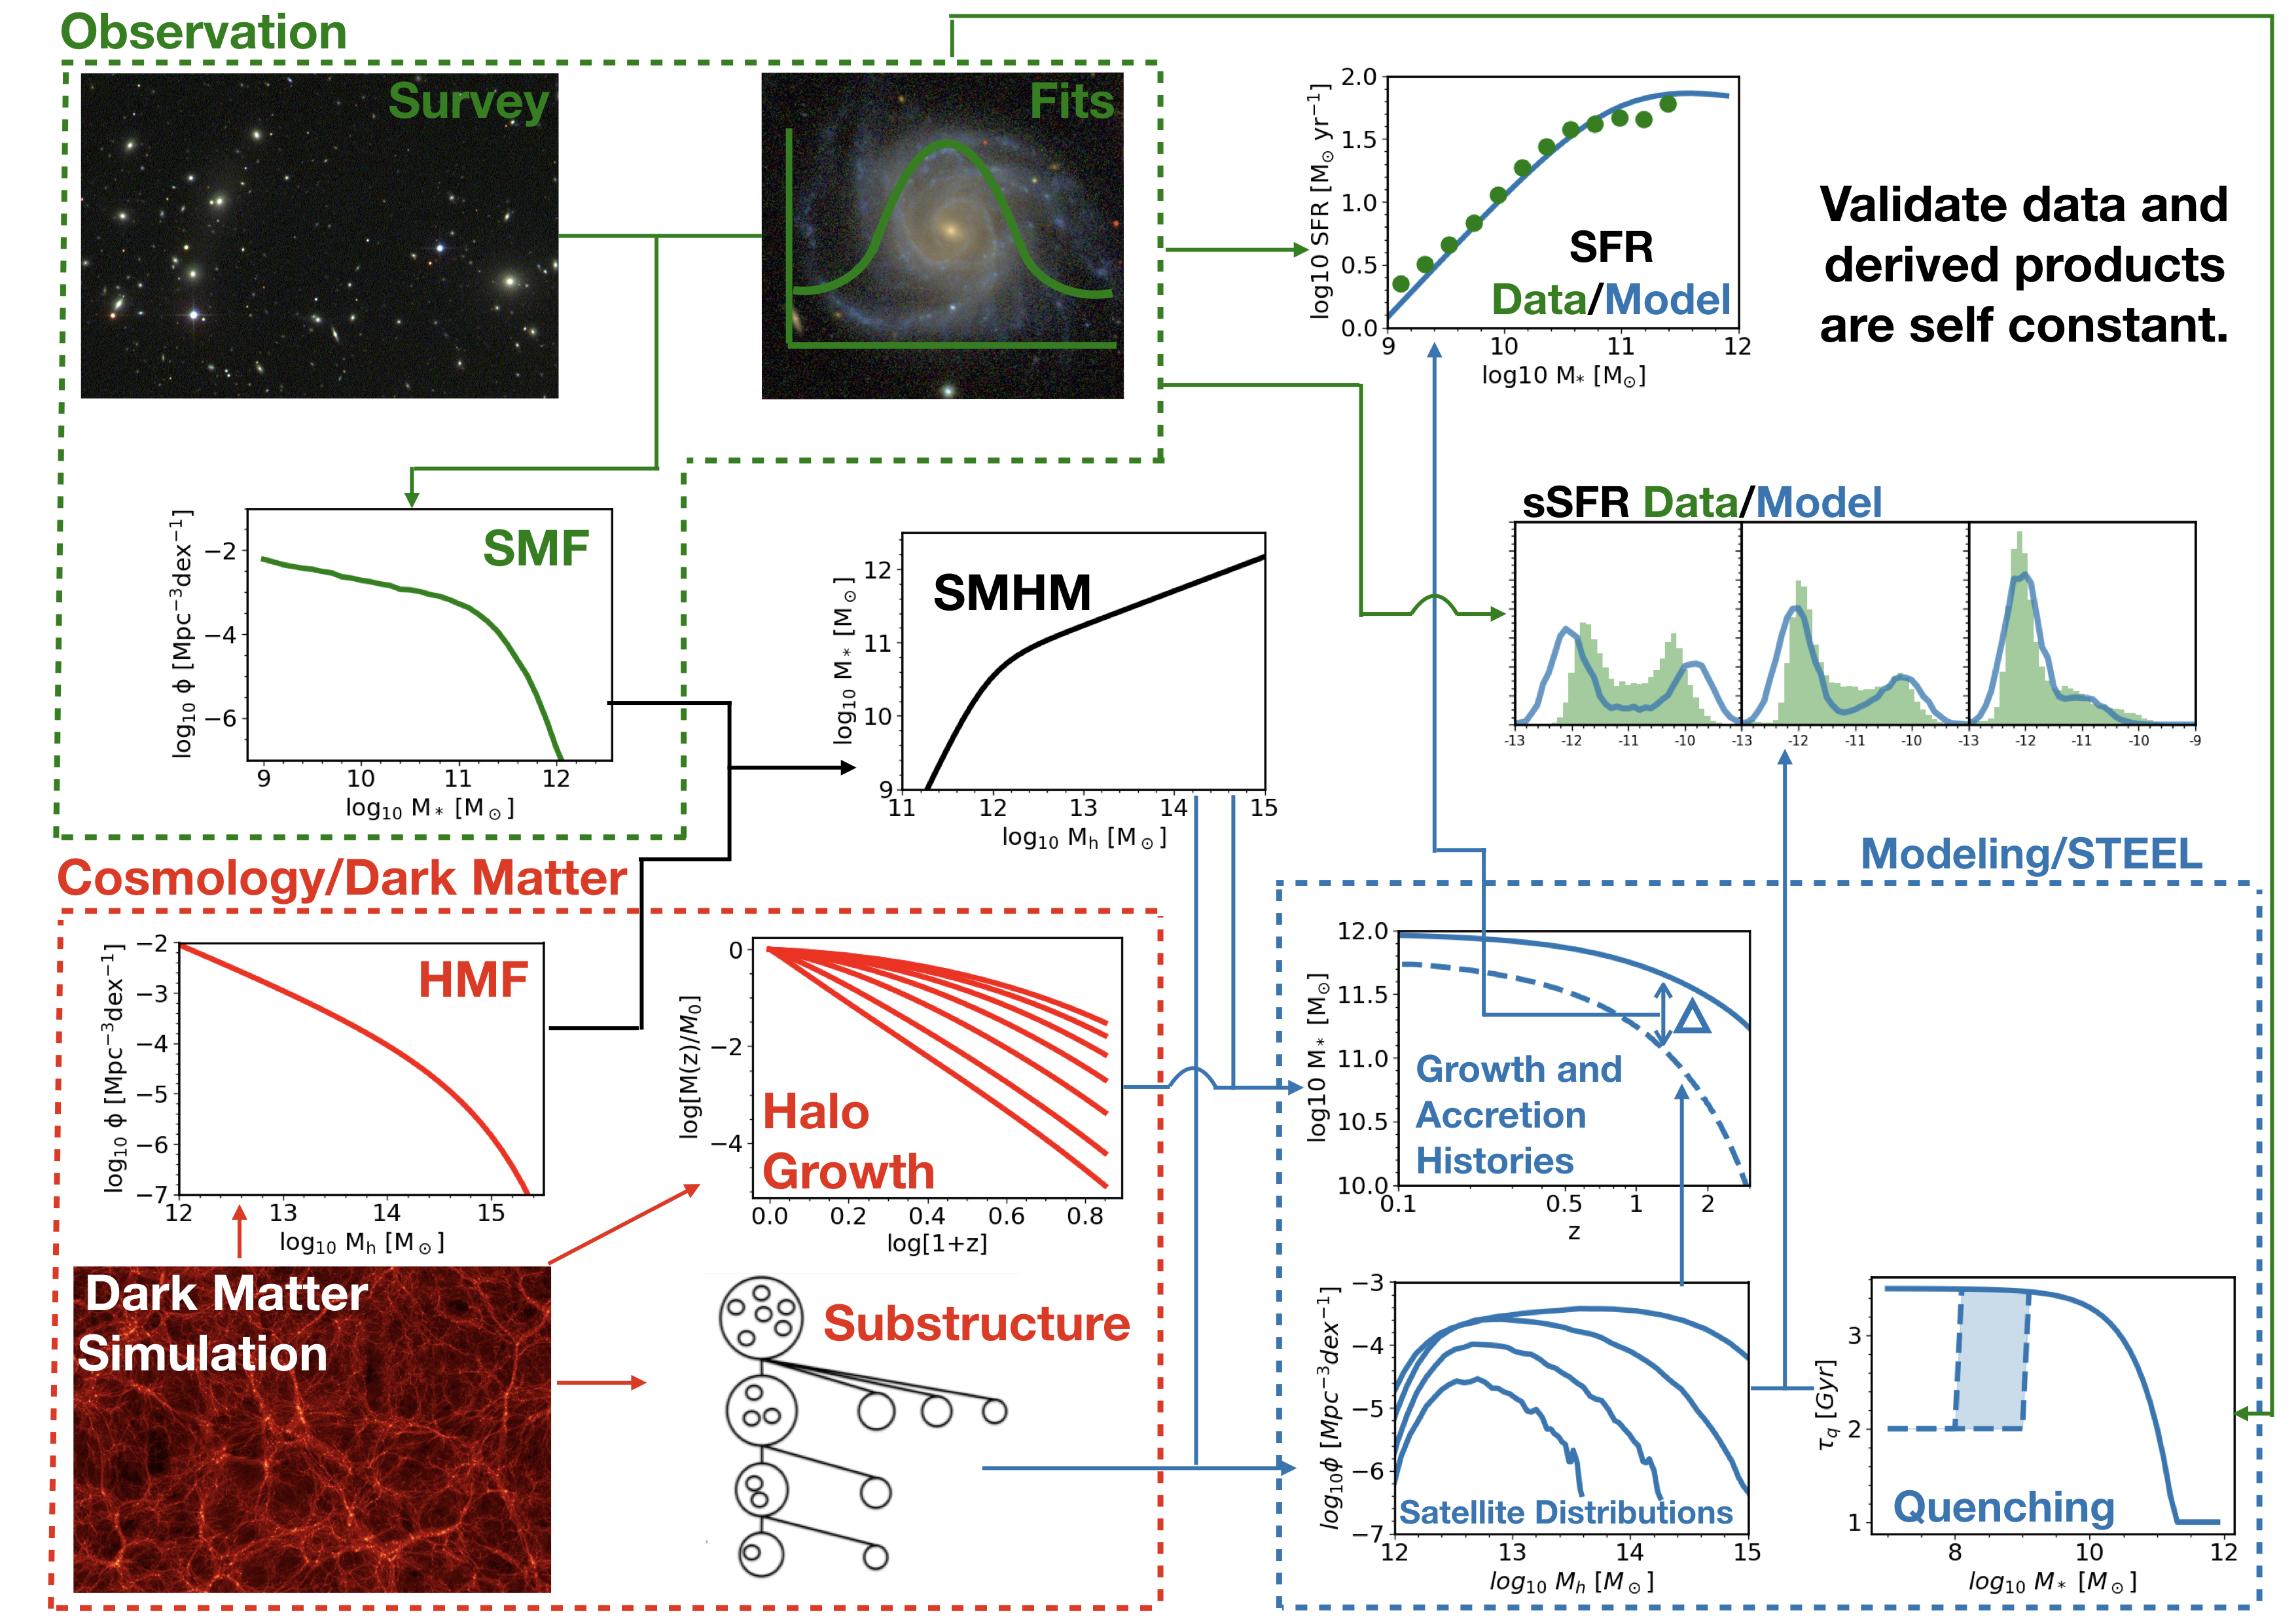
\includegraphics[width = \linewidth]{Figures/Chapter6/FullModelCartoon.png}
    \caption{Schematic cartoon related to Figure \ref{fig:SFRDerevation_Cartoon} of how \steel can be used to check self-consistency between fitting models used on observed data and the theoretical assumptions that underpin the fitting models.}
    \label{fig:Full_Mod_Toon}
\end{figure}
Items closer to the top of the list are less effected by the modelling and therefore likely to be more robust within this method. Often the empirical technique draws on observation to inform modelling, for example the quenching model from \citet{Wetzel2013GalaxyUniverse}, therefore this approach may well present an iterative loop. Using this approach any mismatch between the observational fit and the modelled property can be addressed from three angles appreciating the uncertainties inherent in fitting, modelling, and cosmology together.

\subsection{Galaxy modelling tool}

The proposition for \steel, or another statistical semi empirical model, to become a staple amoungst other competitive galactic modelling tools is based exclusively on the concept of a statistical dark matter accretion history. 

%where is the low hanging fruit?
%how can STEEL become a staple model such as UniM or Illistris?